\documentclass[tikz,border=3pt]{standalone}
\usepackage[T1]{fontenc}
\usepackage{amsmath}
\usepackage{XCharter}
\usepackage[xcharter]{newtxmath}
\usepackage[scaled=.92]{helvet}
\usepackage{pgfplots}
\usetikzlibrary{arrows.meta,positioning,fit,calc,backgrounds,decorations.pathreplacing,patterns}
\usepgfplotslibrary{groupplots,fillbetween}
\pgfplotsset{compat=1.18}
\definecolor{ink}{HTML}{172536}
\definecolor{rgb}{HTML}{3563B8}
\definecolor{event}{HTML}{17857C}
\definecolor{fusion}{HTML}{76529C}
\definecolor{reference}{HTML}{8994A3}
\definecolor{warn}{HTML}{AC5948}
\definecolor{muted}{HTML}{657183}
\definecolor{rule}{HTML}{D9E0E8}
\definecolor{pale}{HTML}{F5F7FA}
\color{ink}
\tikzset{box/.style={rounded corners=2pt,draw=rule,fill=white,align=center,inner sep=4pt,font=\sffamily\fontsize{9}{10.8}\selectfont,minimum height=9mm},rb/.style={box,draw=rgb!50,fill=rgb!5},eb/.style={box,draw=event!50,fill=event!5},fb/.style={box,draw=fusion!55,fill=fusion!5},arrow/.style={-{Latex[length=1.8mm]},line width=.65pt,draw=muted},note/.style={font=\sffamily\fontsize{8.4}{10.2}\selectfont,align=center,text=muted},heading/.style={font=\sffamily\fontsize{10}{12}\selectfont\bfseries,align=left,text=ink}}
\pgfplotsset{paper/.style={width=15.7cm,height=6cm,axis lines*=left,axis line style={rule},tick style={draw=none},tick label style={font=\sffamily\fontsize{8.8}{10.4}\selectfont,text=muted},label style={font=\sffamily\fontsize{9.4}{11}\selectfont,text=ink},title style={font=\sffamily\fontsize{10}{12}\selectfont\bfseries,text=ink},legend style={draw=none,fill=none,font=\sffamily\fontsize{9}{11}\selectfont,cells={anchor=west}},grid=major,grid style={rule!65,line width=.3pt},minor tick num=0,scaled ticks=false,unbounded coords=jump,clip mode=individual}}
\begin{document}

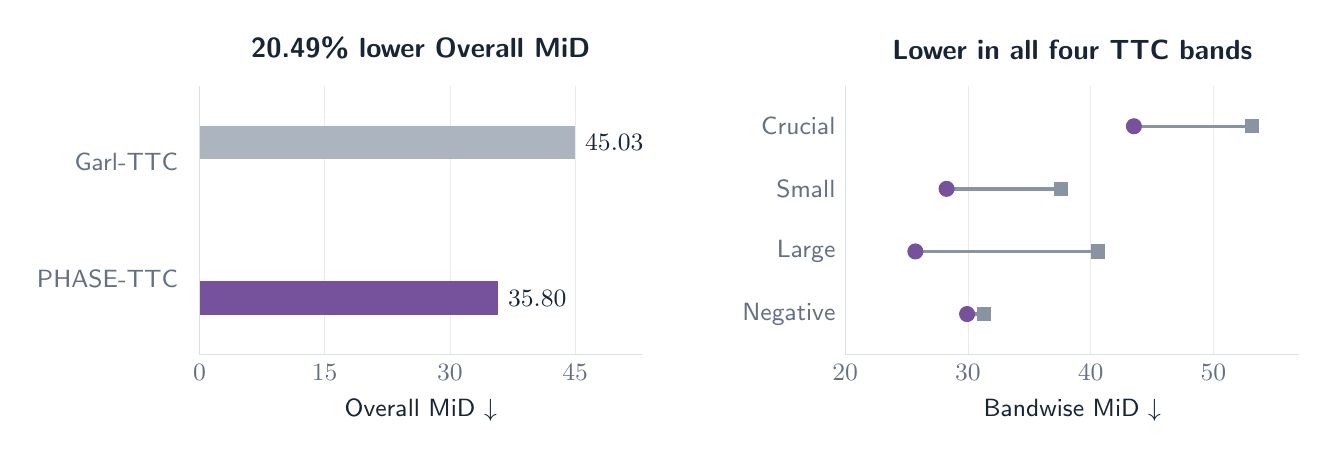
\begin{tikzpicture}

\begin{axis}[paper,at={(0,0)},anchor=south west,width=7.2cm,height=5.0cm,title={20.49\% lower Overall MiD},xbar,bar width=12pt,xmin=0,xmax=53,ymin=-.65,ymax=1.65,ytick={0,1},yticklabels={PHASE-TTC,Garl-TTC},xlabel={Overall MiD \(\downarrow\)},xtick={0,15,30,45},ymajorgrids=false,nodes near coords,nodes near coords style={font=\sffamily\small,text=ink,/pgf/number format/fixed,/pgf/number format/fixed zerofill,/pgf/number format/precision=2},enlarge y limits=false]
\addplot[fill=fusion,draw=none] coordinates {(35.8014515808239,0)};
\addplot[fill=reference!70,draw=none] coordinates {(45.03,1)};
\end{axis}
\begin{axis}[paper,at={(8.2cm,0)},anchor=south west,width=7.35cm,height=5.0cm,title={Lower in all four TTC bands},xmin=20,xmax=57,ymin=-.65,ymax=3.65,ytick={0,1,2,3},yticklabels={Negative,Large,Small,Crucial},xlabel={Bandwise MiD \(\downarrow\)},xtick={20,30,40,50},ymajorgrids=false]
\addplot[reference,line width=1.2pt] coordinates {(29.9313941143029,0) (31.29,0)};
\addplot[reference,line width=1.2pt] coordinates {(25.7178970092572,1) (40.61,1)};
\addplot[reference,line width=1.2pt] coordinates {(28.2567523239348,2) (37.58,2)};
\addplot[reference,line width=1.2pt] coordinates {(43.5189935425749,3) (53.13,3)};
\addplot[only marks,mark=*,mark size=2.7pt,fusion] coordinates {(29.9313941143029,0) (25.7178970092572,1) (28.2567523239348,2) (43.5189935425749,3)};
\addplot[only marks,mark=square*,mark size=2.4pt,reference] coordinates {(31.29,0) (40.61,1) (37.58,2) (53.13,3)};
\end{axis}
\end{tikzpicture}
\end{document}
